\documentclass[preprint]{elsarticle}

% Packages for math
\usepackage{amsmath}
\usepackage{amsfonts}
\usepackage{amssymb}

% Set page margins
\usepackage[letterpaper, left=1in, right=1in, top=1in, bottom=1in]{geometry}
\usepackage{lineno}
\usepackage[capitalize]{cleveref}
\creflabelformat{equation}{#2\textup{#1}#3}
\crefdefaultlabelformat{#2\textup{#1}#3}
\usepackage{tabularx}
\usepackage{mlmodern}
\usepackage{mdframed}
\usepackage{setspace}
\biboptions{sort&compress}


\journal{Computers in Biology and Medicine}
\begin{document}
\setstretch{2}
\linenumbers

\begin{frontmatter}
	\title{3D/2D Projected Shape Sensitivity Analysis of Total Joint Arthroplasty Implants}
	\author[a]{Andrew James Jensen}
	\author[a]{Scott A. Banks}
	\affiliation[a]{
		organization={Mechanical and Aerospace Engineering, University of Florida},
		city={Gainesville},
		state={Florida},
		country={USA}
	}
	\begin{abstract}
  Abstract Placeholder
\end{abstract}

%%% Local Variables:
%%% mode: latex
%%% TeX-master: "../Jensen_Shape_Sensitivity"
%%% End:

	\begin{keyword}
		Computer vision \sep TKA \sep rTSA \sep Shape Descriptor \sep Angular Radial Transform
	\end{keyword}
\end{frontmatter}

\section{Introduction}


The application of Joint Track Machine Learning to reverse Total Shoulder Arthroplasty (rTSA) implants has unfolded a complex scenario.
It highlights the intricate relationship between optimization algorithm performance, specific cost functions, and the inherent shape of the 3D models used for registration.
A particular challenge lies in the intrinsic properties of humeral models, which present unique difficulties in model-image registration.
To address these challenges, a thorough understanding of the relationship between a 3D shape and its projective geometry is crucial.
This understanding is expected to shed light on the stark differences in algorithmic performance between total knee arthroplasty (TKA) and rTSA implants.


Understanding shape and its salient features has been a crucial aspect of computer vision since it was intertwined with psychology and neurology \cite{attneaveInformationalAspectsVisual1954,attneaveQuantitativeStudyShape1956}.
Many intuitively appealing ideas about shape, such as the salience of curvature and vanishing points in projections, required mathematical definition to be effectively incorporated into image processing algorithms.
Invariant Shape Descriptors, which remain consistent across rigid transformations or scaling, are particularly significant \cite{zhangReviewShapeRepresentation2004}.
These descriptors encapsulate the essence of a shape, independent of factors like rotation, scaling, or position in an image.
Normalized Fourier Descriptors are among the most notable examples of invariant shape descriptors that have been used for aircraft recognition \cite{wallaceEfficientThreedimensionalAircraft1980,wallaceAnalysisThreedimensionalMovement1980,richardIdentificationThreeDimensionalObjects1974}, aerial photography classification \cite{linClassificationPartial2D1987}, model-image registration \cite{zossoBiplanar2Dto3DRegistration2008}, and even measuring TKA kinematics from single-plane images \cite{banksAccurateMeasurementThreedimensional1996}.
Hu moments \cite{huVisualPatternRecognition1962}, the Hough Transform \cite{ballardGeneralizingHoughTransform1981}, Shape Context \cite{belongieShapeMatchingObject2002}, Curvature scale space \cite{koenderinkSurfaceShapeCurvature1992}, the Angular Radial Transform \cite{leeNewShapeDescription2012}, and multi-scale Shape Descriptors \cite{al-thelayaInShaDeInvariantShape2021} have all been proposed as robust methods for vectorizing a shape into mathematically comparable elements.

The central inquiry of this chapter is whether a robust binary shape descriptor can elucidate the relative underperformance of model-image registration for rTSA implants compared to TKA implants. This question not only addresses a specific technical challenge but also aims to contribute to the broader understanding of shape analysis in medical imaging.

	{\Large New Introduction}\\
Understanding the in-vivo kinematics of total joint replacement has been a crucial factor in implant design, post-operative assessment, and predictive modeling for wear and failure patterns for nearly 30 years \cite{freglyComputationalWearPrediction2005,banks2003HapPaul2004,banksRationaleResultsFixedBearing2019}.
Recent advancements in computer vision and machine learning and enabled these measurements to occur for total knee arthroplasty (TKA) in a fully autonomous and clinically practical setting utilizing single-plane fluoroscopy \cite{brobergValidationMachineLearning2023,jensenJointTrackMachine2023}.
Unfortunately, there are inherent limitatons in using only a single camera, namely, the loss of depth perception and the introduction of ambiguous projected shapes during optimization \cite{floodAutomatedRegistration3D2018,mahfouzRobustMethodRegistration2003,zuffiModelbasedMethodReconstruction1999,banksAccurateMeasurementThreedimensional1996}.
For mediolaterally symmetric tibial implants, this caused a phenomena dubbed ``symmetry traps'', wherein two distinct 3D orientations of the implant would produce indistinguishable 2D projected geometry.
Symmetry traps were solved by introducing a machine learning algorithm trained on true anatomic orientations that label and correct images that fell into such an optimization minima \cite{jensenCorrectingSymmetricImplantInReview}.
However, this solution still required that the symmetric implant optimize to one of the two potential local minima corresponding to the ``symmetry trap''.

Unfortunately, when this same optimization routine and cost function \cite{floodAutomatedRegistration3D2018,jensenJointTrackMachine2023} was applied to reverse total shoulder arthroplasty (rTSA) it significantly underperformed compared to total knee arthroplasty implants.
The optimization often failed in two ways.
The first was error along the internal/external rotation axis, representing the axis of near-rotational symmetry, as well as the axis whose features are most often occluded by the glenospehere implant in frontal-plane fluoroscopy.
The second was a distal shift of the implant such that the local minima found properly registered the humeral stem, but not the humeral cup.
This led to a deeper exploration of the psychology of shape \cite{attneaveInformationalAspectsVisual1954,attneaveQuantitativeStudyShape1956}, which highlights the importance of relatively high curvature as being the most salient features in binary shape, and binary distance metrics \cite{reinkeCommonLimitationsImage2023,reinkeUnderstandingMetricrelatedPitfalls2023}, which stresses the importance of fitting the cost-function metric to the problem at hand based on the underlying structure of your data.

To incorporate regions of high curvature into a novel-cost function, Menger's discrete curvature algorithm \cite{legerMengerCurvatureRectifiability1999} was applied to the contour of the projected implant shape.
High curvature regions were selected algorithmically, and implemented in a \emph{Modified Asymmetric Surface Distance}, using only the high-curvature keypoints as surface points (\cref{eq:curv-keypoint}).
Unfortunately, this too yielded sub-par results when applied to rTSA humeral implants, falling into the same errors as before.


\begin{equation}
	\label{eq:curv-keypoint}
	\begin{split}
		\displaystyle J & = \dfrac{\sum_{k \in \mathbb{K}}(\min_{p\in Proj}(p \cdot DM_{k}))}{N} \\
		                & \text{where}                                                           \\
		\mathbb{K}      & = \text{Set of all keypoints}                                          \\
		N               & = \text{Number of keypoints}                                           \\
		DM_{k}          & = \text{Distance map for keypoint $k$}                                 \\
		p               & = \text{Single point on projection silhouette}
	\end{split}
\end{equation}

To improve the previously implemented Hamming Distance \cite{jensenJointTrackMachine2023,floodAutomatedRegistration3D2018}, which is always maximally incorrect when there is no overlap, regardless of how close or far the estimate is, we introduce a \emph{Modified Mean Surface Distance}.
To do so, the element-wise multiplication of the projection estimate ($Proj_{x,y}$) and the distance map of the target ($DM_{x,y}$) is taken as a cost function (\cref{eq:DMCF}).
This too, yielded sub-par performance.
\begin{equation}
	\label{eq:DMCF}
	J = \dfrac{ \sum_{(x,y) \in \text{Image}} Proj_{x,y}DM_{x,y} }{\sum_{(x,y)\in \text{Image}}Proj_{x,y}}
\end{equation}

%%% Local Variables:
%%% mode: latex
%%% TeX-master: "../Jensen_Shape_Sensitivity"
%%% End:

\section{Methods}

\subsection{Data Collection}
First, we collected one manufacturer-provided model from each of: rTSA humeral implant, rTSA glenosphere implant, TKA femoral implant, and TKA tibial implant for testing shape sensitivity.
\subsection{Image Generation}
The binary silhouette of each implant was rendered using an in-house CUDA camera model (CUDA Version 12.1) \cite{nickollsScalableParallelProgramming2008} to a $1024\times 1024$ image plane.
The focal length of the pinhole camera model was 1000mm and each pixel was 0.3mm.
All CUDA programming was performed on an NVIDIA Quadro P2200 GPU.
\subsection{Invariant Angular Radial Transform}
The invariant angular radial transform descriptor (IARTD) was selected due to its sensitivity in the radial direction \cite{leeNewShapeDescription2012}.
This sensitivity allows us to address minor changes along the contour of our projected shape, which is a desirable property for determining the minor changes in shape with respect to input orientation.

The IARTD is a complex moment calculated by summing orthogonal basis components on the unit polar disk.
Each basis function has an order ($n$) and a repetition ($p$).
Intuitively, the order represents concentric ``rings'' in our polar disk, and the repetition is the number of ``pie slices'' in our unit disk along $\theta$.
To perform these calculations, we normalize our image such that $(0,0)$ is at the center and $(\pm1,\pm1)$ are the four corners.

Each angular radial transform (ART) coefficient is a complex double integral (\cref{eq:F_np}) over the image in polar coordinates, $f(\rho,\theta)$ multiplied by the ART basis function, $V_{np}(\rho,\theta)$ (\cref{eq:V_np}).

\begin{equation}
	\label{eq:F_np}
	F_{np} = \int_{0}^{2\pi}\int_{0}^{1}f(\rho,\theta)V_{np}(\rho,\theta)\rho d\rho d\theta
\end{equation}

\begin{equation}
	\label{eq:V_np}
	V_{np}(\rho,\theta) = A_{p}(\theta)R_{n}(\rho)
\end{equation}

Our radial basis function is comprised of a complex exponential, $A_{p}(\theta)$ (\cref{eq:A_p}), which provides rotational invariance, and a trigonometric transform, $R_{p}(\theta)$ (\cref{eq:R_n}) to provide orthogonality.

\begin{equation}
	\label{eq:A_p}
	A_{p}(\theta) = \dfrac{1}{2\pi}e^{jp\theta}
\end{equation}
\begin{equation}
	\label{eq:R_n}
	R_{n}(\rho) =
	\begin{cases}
		1                   & n=0     \\
		2 \cos (\pi n \rho) & n \ne 0
	\end{cases}
\end{equation}

Lastly, in order to correct for differences in the in-plane rotation, we apply a phase-correction to each ART coefficient (\cref{eq:art_phase_correction}, \cref{eq:fnp_phase_correction}).
\begin{equation}
	\label{eq:art_phase_correction}
	\phi'_{np} = \phi_{np} - \phi_{n,1}
\end{equation}

\begin{equation}
	\label{eq:fnp_phase_correction}
	F_{np}' = F_{np}e^{-jp\phi_{n,1}}
\end{equation}

And the, the final feature vector becomes a the polar decomposition of our coefficient at each order and repetition \cref{eq:iartd}.
We exclude values from the first two repetitions because they contain no valuable information.
To construct the full IARTD feature vector, we used values of $n=\{0, \dots, 3 \}$ and $p=\{0, \dots, 8\}$.

\begin{equation}
	\label{eq:iartd}
	IARTD = \{|F'_{np}|, \phi_{np}'\} \text{ where } n \ge 0, p \ge 2
\end{equation}

\subsection{Shape Differences and Sensitivity}
The primary goal of this section is to establish a easily interpretable value that captures the overall change from one shape to another.
For clarity in representation, successive rotations were denoted as subscripts, such that $R_{z}R_{x}R_{y} = R_{z,x,y}$. The application of the IARTD equation to an implant at a specific input orientation $R_{z,x,y}$ was represented as $IARTD(R_{z,x,y})$.
Shape differences were calculated using the central difference equation on the IARTD vector produced from two different orientations.
The grid of sampled orientations had extrema of $\pm 30$ with a step size of $5$ for each of the $x$, $y$, and $z$ axes.
The ``differences'' along each axes were computed by applying a positive and negative rotation ($\pm \delta $) of 1 degree.
And so, for every input $x,y,z$ rotation, there will be three shape differences, one for each $\delta_{x}$, $\delta_{y}$ or $\delta_{z}$ (\cref{eq:shape-derivative}).
For notational brevity, we will condense the full equation down to a single $\Delta S(\delta)$, (representing $\Delta Shape$ for a differential rotation $\delta$).

\begin{equation}
	\label{eq:shape-derivative}
	\Delta S(\delta)_{z,x,y} \equiv \dfrac{ \partial IARTD(R_{z,x,y}) }{\partial \delta} \propto IARTD(R_{z,x,y,+\delta}) - IARTD(R_{z,x,y,-\delta})
\end{equation}

Because each element of the IARTD vector is at a different scale, we must standardize each element in order to ensure accurate assessment of global behavior without analysis being dominated by a single value.
We use z-score to do this, which assumes a normal distribution, but allows for some outliers if they are present.


After z-scaling, we took the Euclidean norm of each $S(\delta)_{z,x,y}$ to capture the total amount of change of that shape for a given differential rotation (\cref{eq:euc_norm}).
Our final step takes advantage of two factors: first, that our in-plane rotations are the first in our Euler sequence ($z$-axis), and second, that this type of rotation does not affect the in-plane shape.
And so, for every $x$ and $y$ input rotation, we average all the values where $x$ and $y$ are held constant as $z$ varies (\cref{eq:z_rot_norm}).
This yields our final values, which we will denote $\mathbb{S}$.
$\mathbb{S}_{x,y}$ will have separate plots for each $x$, $y$, and $z$ differential rotation and for each of the four implants.
These plots will be compared with respect to JTML optimization performance and regions of difficulty for optimization.


\begin{equation}
	\label{eq:euc_norm}
	\|S(\delta)_{z,x,y}\|_{2}
\end{equation}

\begin{equation}
	\label{eq:z_rot_norm}
	\mathbb{S}(\delta)_{x,y} = \dfrac{\sum_{z} \| S(\delta)_{z,x,y} \|_{2}}{N}
\end{equation}

%%% Local Variables:
%%% mode: latex
%%% TeX-master: "../main"
%%% TeX-master: "../main"
%%% End:

\section{Results}
The humeral implant exhibited the lowest mean $\mathbb{S}(\delta_{y})$ across all implant types (\cref{fig:hum_sensitivity_plot}) (\cref{tab:ss-vals}).
This rotation represents the final rotation in our Euler rotation sequence (Z-X-Y) and captures the internal/external rotation of the humeral implant.
Additionally, the surface plotted by the humeral shape sensitivity for all $\delta_{x,y,z}$ is much smoother than any of the other plots, demonstrating the relative lack of shape difference for a wide range of input orientations.
Several plots showed regions with relatively low sensitivity.
Specifically, the glenosphere's $\delta_{y}$ sensitivity along the $y=0$ axis (\cref{fig:sca_sensitivity_plot}) and the tibial implant's $\delta_{y}$ sensitivity along the $x=0$ axis (\cref{fig:tib_sensitivity_plot}).
The femoral implant had the highest average sensitivity ($\frac{\mathbb{S}(\delta_{x}) +\mathbb{S}(\delta_{y}) +\mathbb{S}(\delta_{z})  }{3}$) among all implant types .


\begin{table}
	\caption{Average projected-shape sensitivity values for each of the implant models.} \label{tab:ss-vals}
	\begin{tabularx}{\linewidth}{|X|X|X|X|}\hline
		{\bf Implant Type} & Average $\mathbb{S}(\delta_{x})$ & Average  $\mathbb{S}(\delta_{y})$ & Average $\mathbb{S}(\delta_{z})$ \\ \hline
		Humeral            & 8.83                             & 4.82                              & 7.08                             \\\hline
		Glenosphere        & 6.37                             & 6.22                              & 4.86                             \\\hline
		Femoral            & 6.88                             & 8.68                              & 4.93                             \\\hline
		Tibial             & 9.0                              & 5.52                              & 3.72                             \\\hline
	\end{tabularx}
\end{table}


\begin{figure}[h!]
	\centering
	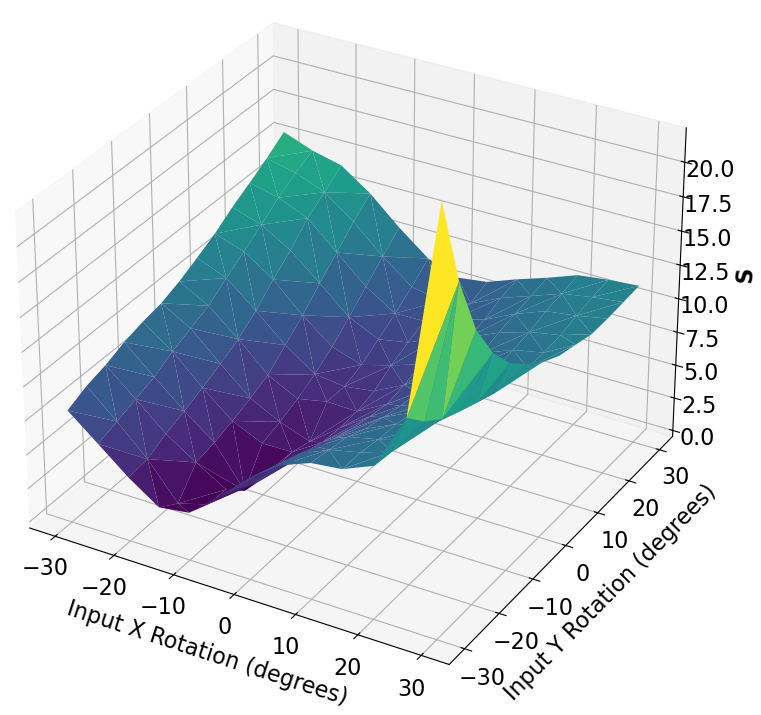
\includegraphics[width=0.3\linewidth]{~/figures/raster/Humeral_dx_sensitivity.png}
	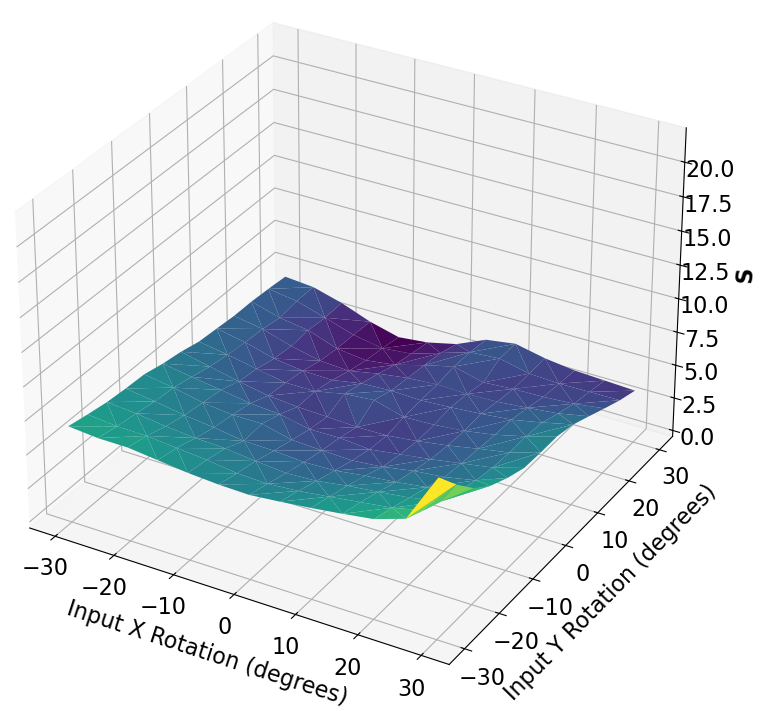
\includegraphics[width=0.3\linewidth]{~/figures/raster/Humeral_dy_sensitivity.png}
	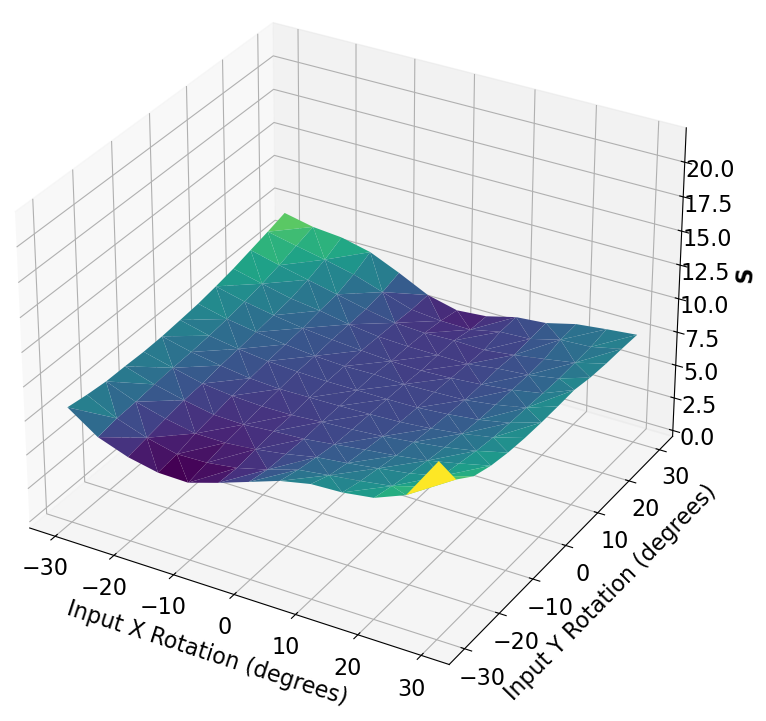
\includegraphics[width=0.3\linewidth]{~/figures/raster/Humeral_dz_sensitivity.png}
	\caption{The $\mathbb{S}$ plot for a humeral implant for $\delta$ rotations along the x, y, and z axis, respectively.}
	\label{fig:hum_sensitivity_plot}
\end{figure}

\begin{figure}[h!]
	\centering
	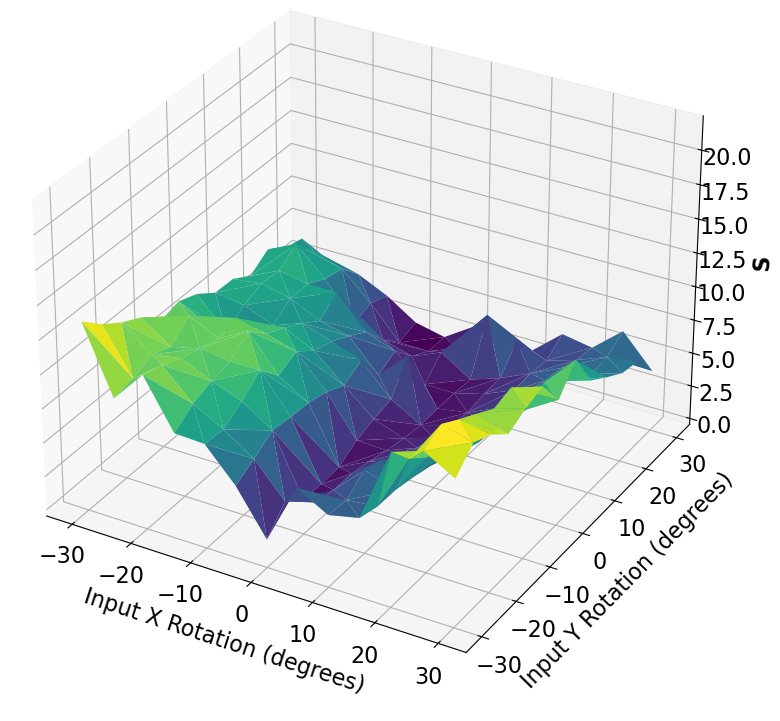
\includegraphics[width=0.3\linewidth]{~/figures/raster/Glenosphere_dx_sensitivity.png}
	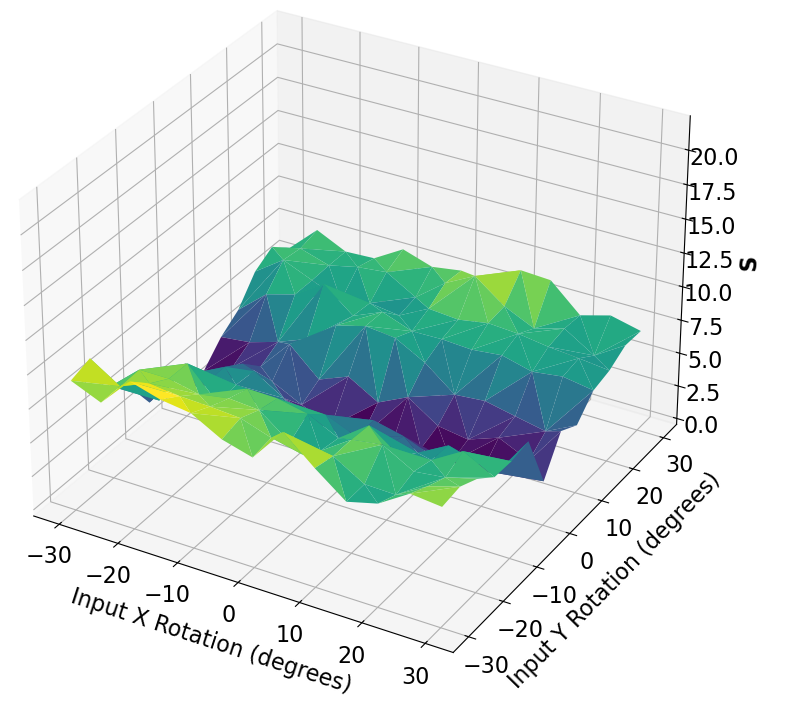
\includegraphics[width=0.3\linewidth]{~/figures/raster/Glenosphere_dy_sensitivity.png}
	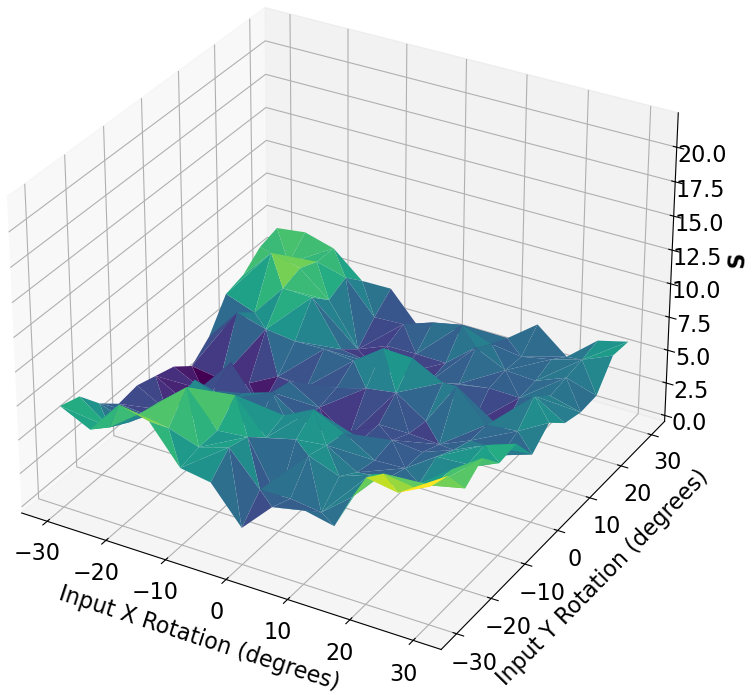
\includegraphics[width=0.3\linewidth]{~/figures/raster/Glenosphere_dz_sensitivity.png}
	\caption{The $\mathbb{S}$ plot for a glenosphere implant for $\delta$ rotations along the x, y, and z axis, respectively.}
	\label{fig:sca_sensitivity_plot}
\end{figure}
\begin{figure}[h!]
	\centering
	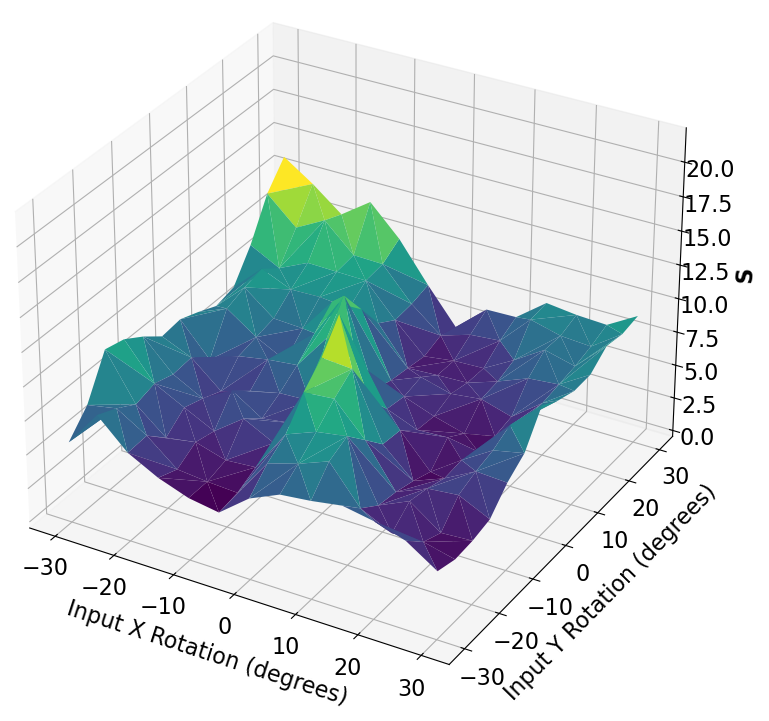
\includegraphics[width=0.3\linewidth]{~/figures/raster/Femoral_dx_sensitivity.png}
	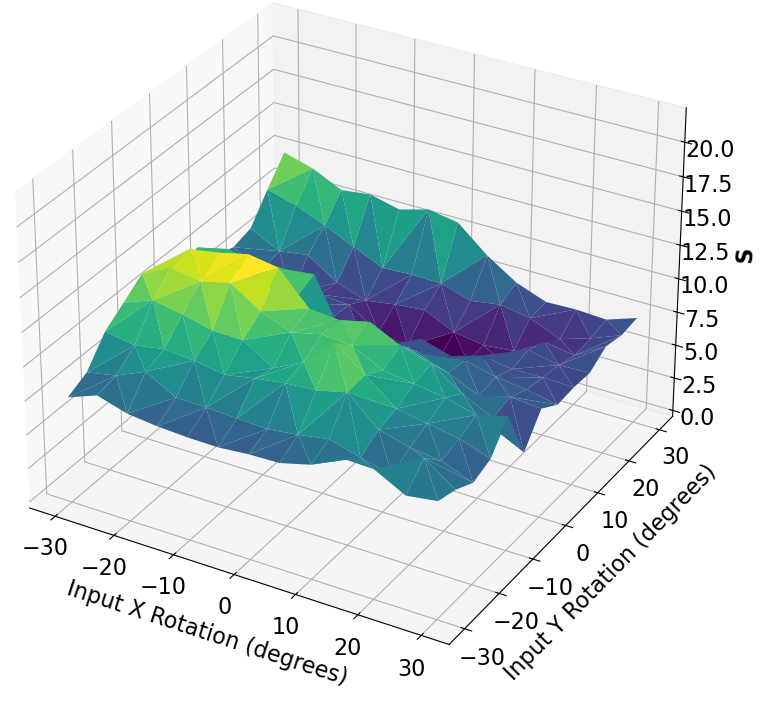
\includegraphics[width=0.3\linewidth]{~/figures/raster/Femoral_dy_sensitivity.png}
	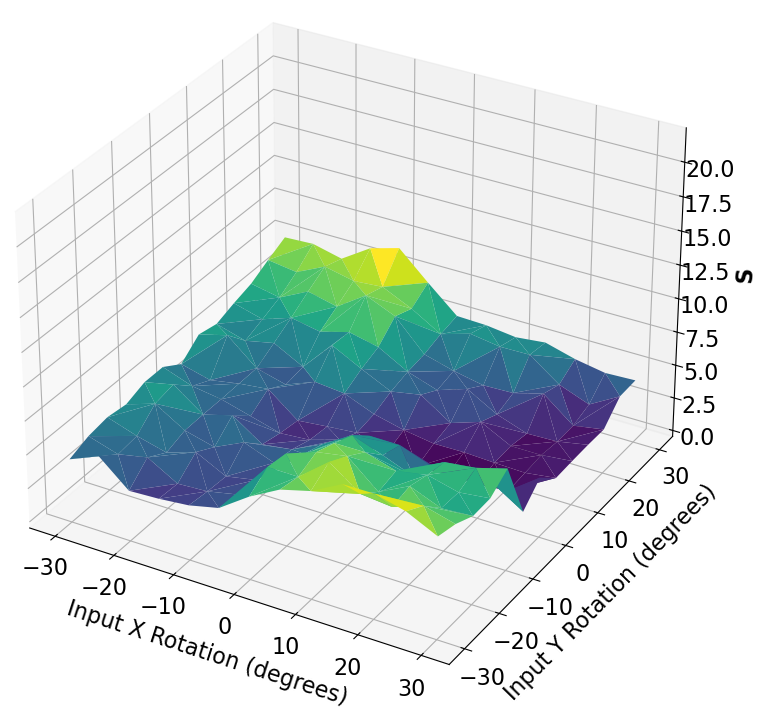
\includegraphics[width=0.3\linewidth]{~/figures/raster/Femoral_dz_sensitivity.png}
	\caption{The $\mathbb{S}$ plot for a femoral implant for $\delta$ rotations along the x, y, and z axis, respectively.}
	\label{fig:fem_sensitivity_plot}
\end{figure}
\begin{figure}[h!]
	\centering
	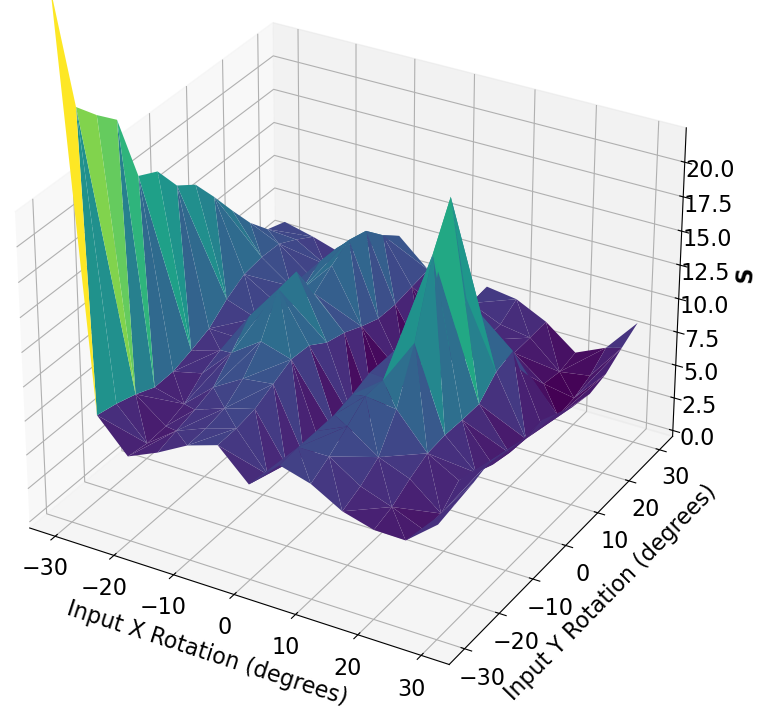
\includegraphics[width=0.3\linewidth]{~/figures/raster/Tibial_dx_sensitivity.png}
	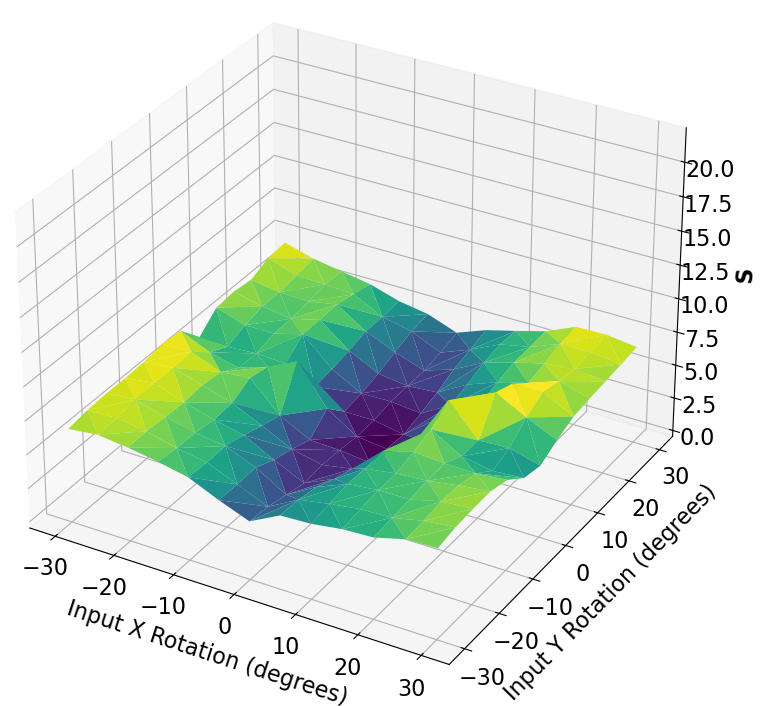
\includegraphics[width=0.3\linewidth]{~/figures/raster/Tibial_dy_sensitivity.png}
	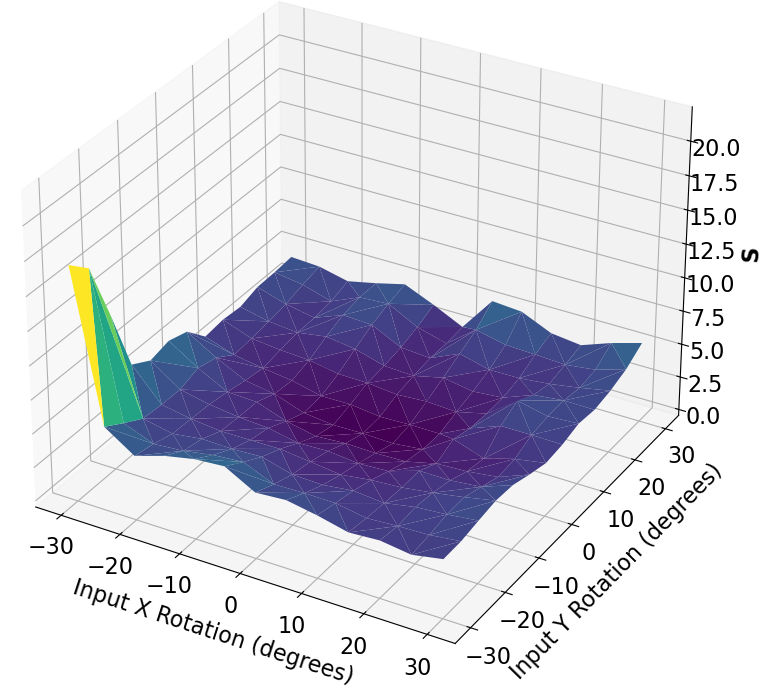
\includegraphics[width=0.3\linewidth]{~/figures/raster/Tibial_dz_sensitivity.png}
	\caption{The $\mathbb{S}$ plot for a tibial implant for $\delta$ rotations along the x, y, and z axis, respectively.}
	\label{fig:tib_sensitivity_plot}
\end{figure}


%%% Local Variables:
%%% mode: latex
%%% TeX-master: "../Jensen_Shape_Sensitivity"
%%% End:

\section{Discussion}
The findings correspond closely with initial expectations regarding the sensitivity measurement of projected shapes relative to 3D object orientation and are consistent with areas challenging for JTML optimization.
Specifically, the humeral implant showed a generally smooth and minimal shape sensitivity profile, particularly for $\delta_{y}$ rotations (\cref{tab:ss-vals}).
Along this axis, the humeral implant is the most cylindrical, meaning we would not expect to see a significant change in the shape descriptor with minor $\delta_{y}$ rotations.
Furthermore, it is noteworthy that this axis presented the most significant difficulties in JTML optimization.

Similar intuitive outcomes are observed with the glenosphere implant, which exhibited the lowest average $\mathbb{S}(\delta)$ among all the implant types.
This implant primarily consists of an articulation surface closely approximating a spherical shape.
Given that the projection of a sphere (a circle) remains constant regardless of the sphere's orientation, the closer a shape is to a spherical form, the lower its overall shape sensitivity is expected to be.

The observed shape sensitivity of the tibial implant with respect to $\delta_{y}$ rotation aligns with the concept of symmetry traps.
There is a consistently low shape sensitivity along the line where $x=0$.
This axis, associated with internal/external rotation, is the same one that contributes to symmetry traps, where two different 3D orientations result in an identical projected shape.
In terms of this analysis, the $\Delta S$ value would be $0$ for these two orientations of the tibial implant.

This study sheds light on an important aspect of Joint Track Machine Learning, particularly the use of Euler angles in the DIRECT-JTA optimization routine.
Currently, the optimization does not involve independently varying all angles within a body-centered reference frame, as this approach is not conducive to hyperbox creation.
Instead, optimization is performed over a range of ordered rotations, projected through the sequence $R_{z}R_{x}R_{y}$.
The challenges the humeral implant encounters in aligning the $y$-axis illustrate that this ordered sequence, especially with a symmetric final axis, can hinder the convergence process.

Beyond the inherent shape sensitivities, such optimization limitations motivate exploring alternatives to Euler angles.
Performing registration optimization directly on the Special Orthogonal group $SO(3)$ poses an intriguing direction.
$SO(3)$ encapsulates all possible 3D rotations in a mathematically convenient structure (A \emph{Lie Group}, which is both a manifold and a group).
By optimizing on this manifold instead of using specific angle parametrizations, issues with gimbal lock and cascade effects can be avoided.
Optimization over Lie groups is an emerging subfield - establishing robust $SO(3)$-based registration cost functions could significantly improve JTML convergence while relying less on descriptor sensitivity along certain axes.

Lastly, incorporating bone information into the optimization routine seems to be the most likely path forward for disambiguating difficult implant orientations.
This study demonstrates that for specific implant geometries, there are inherent limitations to the information that can be gathered from the projected 2D shape as manifest in fluoroscopic imaging.
Utilizing bone information, such as keypoints representing specific anatomic structures, would drastically increase the amount of information present during optimization, and could offer robust constraints on the possible 3D orientations of implant models.



%%% Local Variables:
%%% mode: latex
%%% TeX-master: "../Jensen_Shape_Sensitivity"
%%% End:

\section{Conclusion}
This study demonstrates intrinsic differences between implant types regarding projected 2D shape sensitivity.
Measurement difficulties aligned with low sensitivity along problematic axes—humeral internal rotation and tibial symmetry traps.
Fundamentally, small orientation changes yielded negligible 2D variability for near-symmetrical geometries and axes.
While inherent shape constraints limit data extractable solely from single-plane fluoroscopic silhouettes, incorporating additional image information like bone offers promise.
Despite unavoidable ambiguity along select dimensions, boosting descriptor sensitivity and employing precise anatomical constraints could enable robust clinical tracking.
Overall, relating optimization performance to shape response underscores routes toward accurate autonomous kinematic analysis.

%%% Local Variables:
%%% mode: latex
%%% TeX-master: "../Jensen_Shape_Sensitivity"
%%% End:


\bibliographystyle{elsarticle-num}
\bibliography{~/org/biblio.bib}

\end{document}
%%% Local Variables:
%%% mode: latex
%%% TeX-master: t
%%% End:
